\renewcommand{\arraystretch}{.5}
\section{Grundformeln}

\begin{longtable}{| p{.35\textwidth} | p{.40\textwidth} |}
    \hline
    Berechnung des Mittelwertes
    &\ $X_{AV} = \frac{1}{T}\int\limits_{0}^{T}x(t)dt$\\
    \hline
    Berechnung des Gleichwertes
    &\ $\overline{|X|} = \frac{1}{T} \int\limits_{0}^{T} |x(t)|dt$\\
    \hline
    Berechnung des Effektivwertes
    &\ $X_{RMS} = \sqrt{\frac{1}{T}\int\limits_{0}^{T}x^2(t)dt}$\\
    \hline
    Effektivwert Oberwellen
    & $X_{RMS\_Oberwellen} = \sqrt{X_{RMS}^2 - X_{AV}^2}$\\
    \hline
    Formfaktor
    & $F = \frac{X_{RMS}}{\overline{|X|}}$\\
    \hline
    Welligkeit
    & $w = \frac{X_{RMS\_Oberwellen}}{|X_{AV}|}= \frac{\sqrt{\sum\limits_{k = 1}^{\infty}X_{k}^2}}{|X_{AV}|} = \sqrt{F^2-1}$\\
    \hline
    Leistungsfaktor&
    $ \lambda = \frac{P}{S} $
    \\ \hline 
\end{longtable}

\begin{longtable}{| p{.15\textwidth} | p{.15\textwidth} | p{.15\textwidth}|}%LAYOUT
    \hline
    &
    \textbf{Formfaktor}&
    \textbf{Crestfaktor}\\ \hline
    
    \tabbild[width=2cm]{images/GFSinus}&
    \[ F=\dfrac{X_{RMS}}{|\overline{X}|} \]&
    \[ C=\dfrac{\hat{X}}{X_{RMS}} \]\\ \hline
    
    \tabbild[width=2cm]{images/GFSinusSinus}&
    \[ \sqrt{2} \]&
    \[ \dfrac{\pi}{2 \sqrt{2}} = 1.11 \]\\ \hline
    
    \tabbild[width=2cm]{images/GFSinusGR}&
    \[ 2 \]&
    \[ \dfrac{\pi}{2} \]\\ \hline

    \tabbild[width=2cm]{images/GFRechteck}&
    \[ \sqrt{\dfrac{T}{\tau}} \]&
    \[ \sqrt{\dfrac{T}{\tau}} \]\\ \hline
    
    \tabbild[width=2cm]{images/GFDreieck}&
    \[ \sqrt{3} \]&
    \[ \dfrac{2}{\sqrt{3}}=1.15 \]\\ \hline
    
\end{longtable}

\subsection{Leistungen}
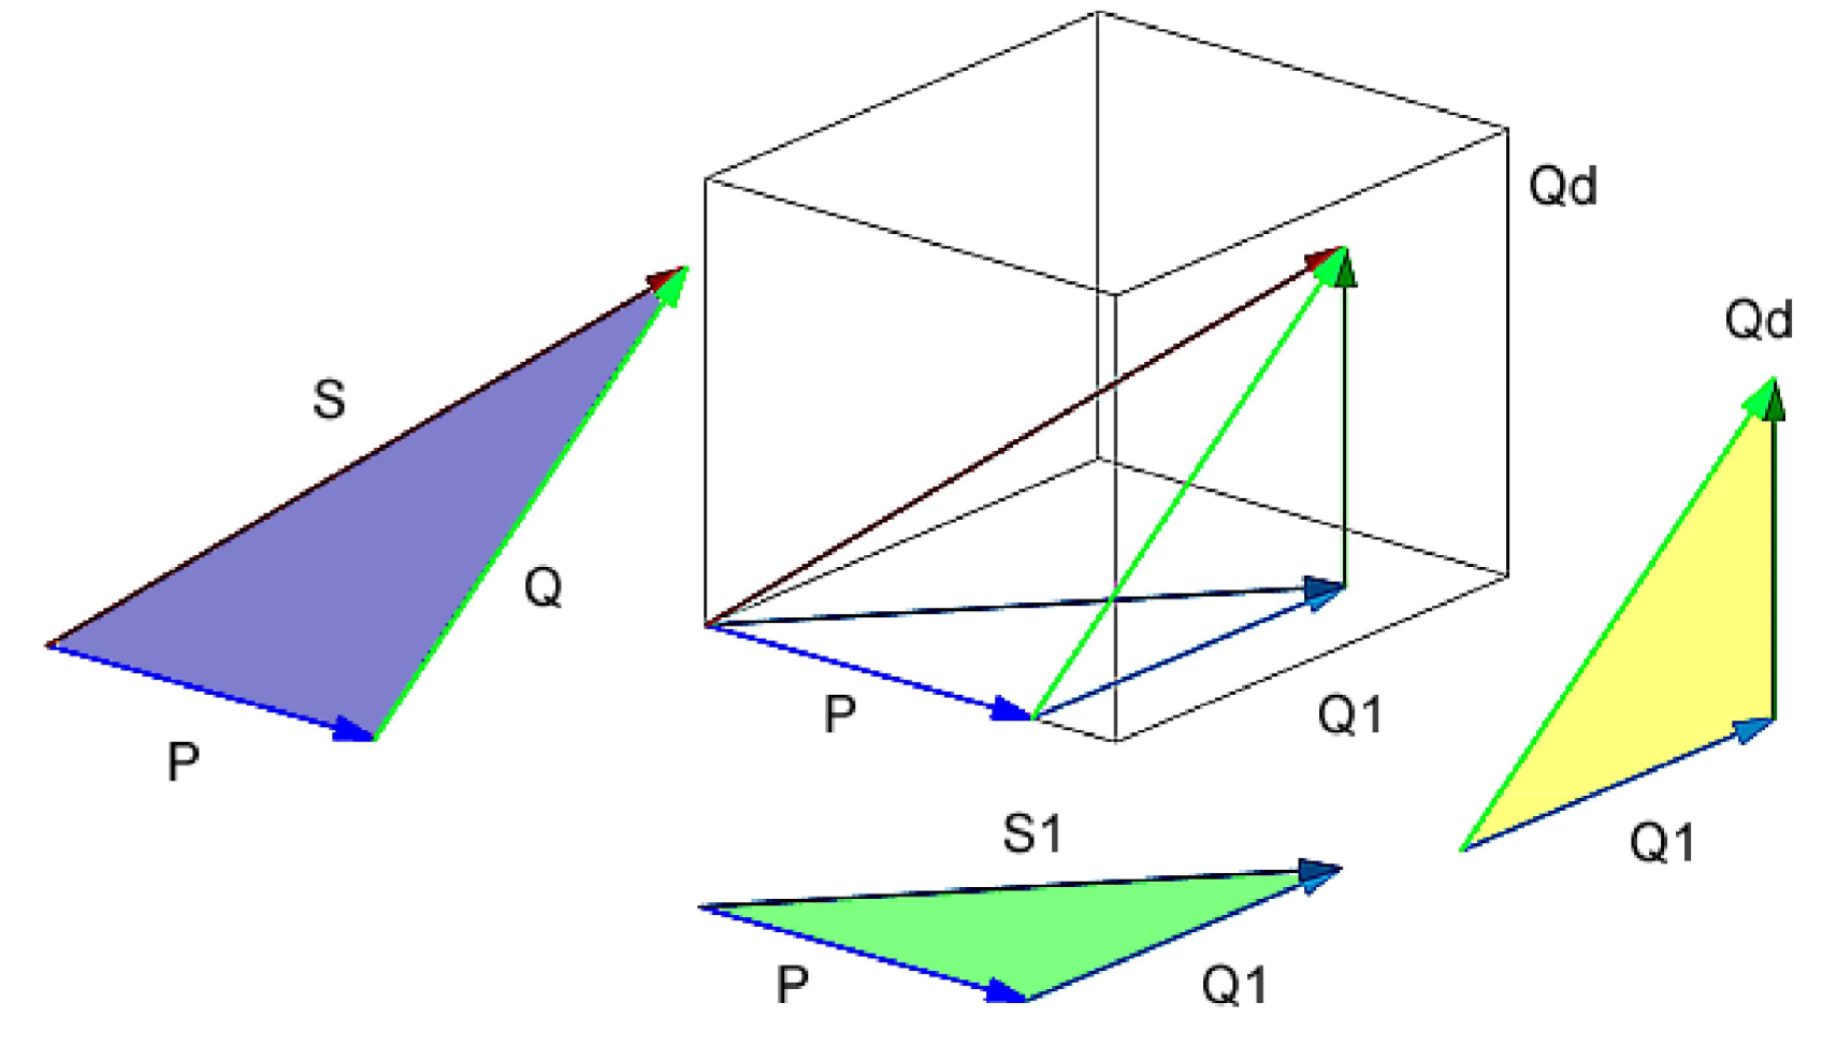
\includegraphics[width=0.4\linewidth]{images/LeistungsDreieck}
\begin{longtable}{| p{.3\textwidth} | p{.40\textwidth} |p{.25\textwidth}|}
    \hline
    
    \textbf{{\color{blue}Scheinleistung}}&
    \[ S=U\cdot I =  \sqrt{P^2+Q^2} = \sqrt{P^2+Q_1^2+Q_d^2} \]&
    \\ \hline
    
    \textbf{Wirkleistung}&
    \[ P=U\cdot I \cdot cos\varphi_1 \]&
    \\ \hline 
       
    \textbf{\color{yellow}Blindleistung}&
    \[ Q=U\cdot I \cdot sin\varphi_1 \]
    \[ Q_1 = S_1 \cdot sin \varphi_1 \]
    \[ Q_d = U\sqrt{\sum_{m=2}^{\infty}I_m^2=\sqrt{Q^2-Q_1^2}} \]&
    $ Q_1 $= Grundschwingungs- \newline \quad Blindleistung\newline
    $ Q_d $= Verzerrungsleistung\newline
    \\ \hline
      
    \textbf{\color{green}Grundschwingungs-\newline scheinleistung}&
    \[ S_1=U_1\cdot I_1 = \sqrt{P^2+Q_1^2} \]&
    $ S_1 $= Grundschwingungs-Scheinleistung
    \\ \hline    
    
    &
    &
    \\ \hline    
    
    &
    &
    \\ \hline   
     
\end{longtable}

%TODO Fourier
\clearpage